\begin{figure}[!t]
  \centering
  \makebox[\linewidth][c]{%
    \resizebox{1.15\linewidth}{!}{%
      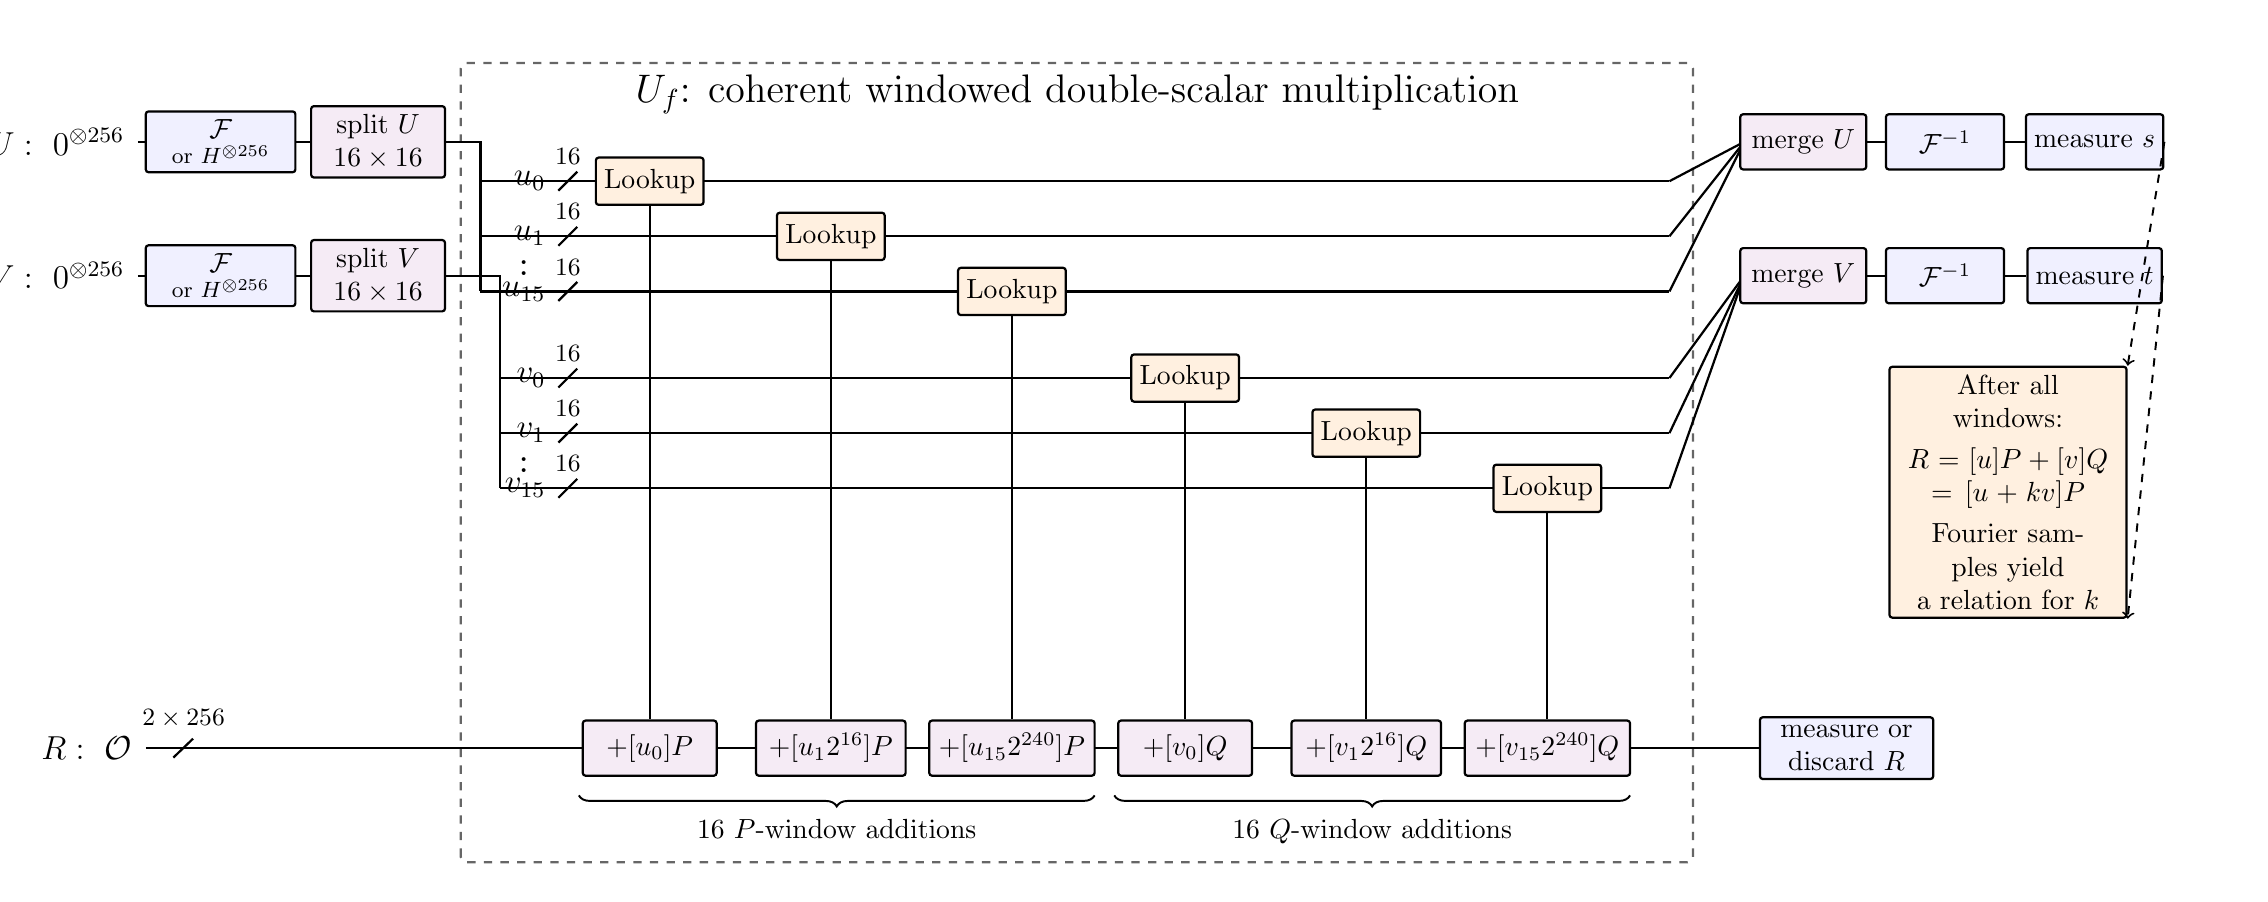
\begin{tikzpicture}[
        x=1cm,
        y=1cm,
        shorwire/.style={black, line width=0.8pt},
        shorgate/.style={draw=black, line width=0.8pt, fill=blue!6,
          minimum height=7mm, rounded corners=1pt, inner sep=3pt,
          align=center, font=\normalsize},
        shorlookup/.style={draw=black, line width=0.8pt, fill=orange!12,
          minimum height=6mm, rounded corners=1pt, inner sep=3pt,
          align=center, font=\normalsize},
        shoradd/.style={draw=black, line width=0.8pt, fill=violet!8,
          minimum height=7mm, rounded corners=1pt, inner sep=3pt,
          align=center, font=\normalsize},
        shorlabel/.style={font=\large},
      ]
        \path[use as bounding box] (0.2,0.25) rectangle (28.3,11.0);

        % Fourier-register preparation.
        \node[shorlabel, anchor=east] at (1.55,9.55)
          {$U:\ \ket{0}^{\otimes256}$};
        \node[shorlabel, anchor=east] at (1.55,7.85)
          {$V:\ \ket{0}^{\otimes256}$};
        \node[shorgate, minimum width=19mm] (fu) at (2.65,9.55)
          {$\mathcal F$\\[-1mm]{\footnotesize or $H^{\otimes256}$}};
        \node[shorgate, minimum width=19mm] (fv) at (2.65,7.85)
          {$\mathcal F$\\[-1mm]{\footnotesize or $H^{\otimes256}$}};
        \node[shorgate, fill=violet!8, minimum width=17mm] (splitu)
          at (4.65,9.55) {split $U$\\$16\times16$};
        \node[shorgate, fill=violet!8, minimum width=17mm] (splitv)
          at (4.65,7.85) {split $V$\\$16\times16$};
        \draw[shorwire] (1.60,9.55) -- (fu.west);
        \draw[shorwire] (1.60,7.85) -- (fv.west);
        \draw[shorwire] (fu.east) -- (splitu.west);
        \draw[shorwire] (fv.east) -- (splitv.west);

        % Coherent double-scalar multiplication boundary.
        \draw[black!60, line width=0.8pt, dashed, rounded corners=2pt]
          (5.70,0.40) rectangle (21.35,10.55);
        \node[font=\Large] at (13.53,10.15)
          {$U_f$: coherent windowed double-scalar multiplication};

        % Representative U-window wires and QROM lookups.
        \foreach \yy in {9.05,8.35,7.65}{
          \draw[shorwire] (6.85,\yy) -- (21.05,\yy);
        }
        \node[shorlabel, anchor=east, fill=white, inner sep=1pt] at (6.82,9.05) {$\ket{u_0}$};
        \node[shorlabel, anchor=east, fill=white, inner sep=1pt] at (6.82,8.35) {$\ket{u_1}$};
        \node[font=\Large] at (6.50,7.98) {$\vdots$};
        \node[shorlabel, anchor=east, fill=white, inner sep=1pt] at (6.82,7.65) {$\ket{u_{15}}$};
        \foreach \yy in {9.05,8.35,7.65}{
          \draw[shorwire] (6.94,\yy-0.12) -- (7.18,\yy+0.12);
          \node[font=\small] at (7.06,\yy+0.31) {$16$};
        }
        \node[shorlookup] (LuZero) at (8.10,9.05) {Lookup};
        \node[shorlookup] (LuOne)  at (10.40,8.35) {Lookup};
        \node[shorlookup] (LuLast) at (12.70,7.65) {Lookup};

        % Representative V-window wires and QROM lookups.
        \foreach \yy in {6.55,5.85,5.15}{
          \draw[shorwire] (6.85,\yy) -- (21.05,\yy);
        }
        \node[shorlabel, anchor=east, fill=white, inner sep=1pt] at (6.82,6.55) {$\ket{v_0}$};
        \node[shorlabel, anchor=east, fill=white, inner sep=1pt] at (6.82,5.85) {$\ket{v_1}$};
        \node[font=\Large] at (6.50,5.48) {$\vdots$};
        \node[shorlabel, anchor=east, fill=white, inner sep=1pt] at (6.82,5.15) {$\ket{v_{15}}$};
        \foreach \yy in {6.55,5.85,5.15}{
          \draw[shorwire] (6.94,\yy-0.12) -- (7.18,\yy+0.12);
          \node[font=\small] at (7.06,\yy+0.31) {$16$};
        }
        \node[shorlookup] (LvZero) at (14.90,6.55) {Lookup};
        \node[shorlookup] (LvOne)  at (17.20,5.85) {Lookup};
        \node[shorlookup] (LvLast) at (19.50,5.15) {Lookup};

        % Compact split buses avoid a dense bundle of diagonal fan-out lines.
        \draw[shorwire] (splitu.east) -- (5.95,9.55) -- (5.95,7.65);
        \foreach \yy in {9.05,8.35,7.65}{
          \draw[shorwire] (5.95,\yy) -- (6.85,\yy);
          \draw[shorwire] (21.05,\yy) -- (22.00,9.55);
        }
        \draw[shorwire] (splitv.east) -- (6.20,7.85) -- (6.20,5.15);
        \foreach \yy in {6.55,5.85,5.15}{
          \draw[shorwire] (6.20,\yy) -- (6.85,\yy);
          \draw[shorwire] (21.05,\yy) -- (22.00,7.85);
        }

        % Accumulator and representative point additions.
        \node[shorlabel, anchor=east] at (1.65,1.85)
          {$R:\ \ket{\mathcal O}$};
        \draw[shorwire] (1.70,1.85) -- (24.20,1.85);
        \draw[shorwire] (2.05,1.73) -- (2.30,1.97);
        \node[font=\small] at (2.18,2.22) {$2\times256$};
        \node[shoradd, minimum width=17mm] (AuZero) at (8.10,1.85)
          {$+[u_0]P$};
        \node[shoradd, minimum width=19mm] (AuOne) at (10.40,1.85)
          {$+[u_1 2^{16}]P$};
        \node[shoradd, minimum width=21mm] (AuLast) at (12.70,1.85)
          {$+[u_{15}2^{240}]P$};
        \node[shoradd, minimum width=17mm] (AvZero) at (14.90,1.85)
          {$+[v_0]Q$};
        \node[shoradd, minimum width=19mm] (AvOne) at (17.20,1.85)
          {$+[v_1 2^{16}]Q$};
        \node[shoradd, minimum width=21mm] (AvLast) at (19.50,1.85)
          {$+[v_{15}2^{240}]Q$};
        \draw[shorwire] (LuZero.south) -- (AuZero.north);
        \draw[shorwire] (LuOne.south)  -- (AuOne.north);
        \draw[shorwire] (LuLast.south) -- (AuLast.north);
        \draw[shorwire] (LvZero.south) -- (AvZero.north);
        \draw[shorwire] (LvOne.south)  -- (AvOne.north);
        \draw[shorwire] (LvLast.south) -- (AvLast.north);
        \draw[decorate, decoration={brace, amplitude=4pt}, line width=0.7pt]
          (13.75,1.25) -- (7.20,1.25)
          node[midway, below=5pt, font=\normalsize] {$16$ $P$-window additions};
        \draw[decorate, decoration={brace, amplitude=4pt}, line width=0.7pt]
          (20.55,1.25) -- (14.00,1.25)
          node[midway, below=5pt, font=\normalsize] {$16$ $Q$-window additions};

        % Fourier readout and classical recovery.
        \node[shorgate, fill=violet!8, minimum width=16mm] (mergeu)
          at (22.75,9.55) {merge $U$};
        \node[shorgate, fill=violet!8, minimum width=16mm] (mergev)
          at (22.75,7.85) {merge $V$};
        \node[shorgate, minimum width=15mm] (ifu) at (24.55,9.55)
          {$\mathcal F^{-1}$};
        \node[shorgate, minimum width=15mm] (ifv) at (24.55,7.85)
          {$\mathcal F^{-1}$};
        \node[shorgate, minimum width=17mm] (mu) at (26.45,9.55)
          {measure $s$};
        \node[shorgate, minimum width=17mm] (mv) at (26.45,7.85)
          {measure $t$};
        \draw[shorwire] (mergeu.east) -- (ifu.west);
        \draw[shorwire] (mergev.east) -- (ifv.west);
        \draw[shorwire] (ifu.east) -- (mu.west);
        \draw[shorwire] (ifv.east) -- (mv.west);
        \node[shorgate, minimum width=22mm] at (23.30,1.85)
          {measure or\\discard $R$};
        \node[shorlookup, text width=28mm, minimum height=22mm] (post)
          at (25.35,5.10)
          {After all windows:\\[1mm]
           $R=[u]P+[v]Q$\\
           $=[u+kv]P$\\[1mm]
           Fourier samples yield\\a relation for $k$};
        \draw[dashed,->,line width=0.7pt] (mu.east) -- (post.north east);
        \draw[dashed,->,line width=0.7pt] (mv.east) -- (post.south east);
      \end{tikzpicture}%
    }%
  }
  \caption{Placement of the point-addition kernel within windowed Shor ECDLP.
  The Fourier registers encode $u$ and $v$ and are split into $16$-bit windows;
  each window coherently selects a precomputed multiple of $P$ or $Q$ and adds
  it to the accumulator, yielding $R=[u]P+[v]Q$ before inverse Fourier
  transforms and measurement. The braces show the $32$ conceptual window
  additions; boundary optimizations reduce the estimate used in this paper to
  $28$ point-addition calls. Submission \texttt{8e9c9a2} implements the
  repeated mixed point-addition kernel; QROM and full-Shor integration are
  shown for context and require separate implementation and validation.}
  \label{fig:windowed-shor-ecdlp-overview}
\end{figure}
